\documentclass[11pt,a4paper]{article}

% Packages
\usepackage[utf8]{inputenc}
\usepackage[T1]{fontenc}
\usepackage{amsmath,amssymb,amsfonts}
\usepackage{geometry}
\usepackage{hyperref}
\usepackage{booktabs}
\usepackage{array}
\usepackage{xcolor}
\usepackage{fancyhdr}
\usepackage{titlesec}
\usepackage{enumitem}
\usepackage{algorithm}
\usepackage{algpseudocode}
\usepackage{tcolorbox}
\usepackage{tikz}
\usetikzlibrary{positioning,arrows.meta,calc}

% Page geometry
\geometry{margin=1in}

% Colors
\definecolor{sectioncolor}{RGB}{30,30,30}
\definecolor{linkcolor}{RGB}{0,51,102}
\definecolor{boxbg}{RGB}{245,245,250}
\definecolor{consensusbg}{RGB}{230,245,230}
\definecolor{cullbg}{RGB}{250,235,235}
\definecolor{polarbg}{RGB}{255,245,230}

% Hyperref setup
\hypersetup{
    colorlinks=true,
    linkcolor=linkcolor,
    urlcolor=linkcolor,
    citecolor=linkcolor
}

% Header/Footer
\pagestyle{fancy}
\fancyhf{}
\rhead{\textit{Resonant Consensus Protocol}}
\cfoot{\thepage}

% Section formatting
\titleformat{\section}{\Large\bfseries\color{sectioncolor}}{\thesection}{1em}{}
\titleformat{\subsection}{\large\bfseries\color{sectioncolor}}{\thesubsection}{1em}{}

% Custom boxes
\newtcolorbox{defbox}[1][]{
    colback=boxbg, colframe=gray!50, fonttitle=\bfseries,
    title=#1, boxrule=0.5pt, arc=2pt
}

\newtcolorbox{greenbox}[1][]{
    colback=consensusbg, colframe=green!40!black, fonttitle=\bfseries,
    title=#1, boxrule=0.5pt, arc=2pt
}

\newtcolorbox{redbox}[1][]{
    colback=cullbg, colframe=red!40!black, fonttitle=\bfseries,
    title=#1, boxrule=0.5pt, arc=2pt
}

\newtcolorbox{orangebox}[1][]{
    colback=polarbg, colframe=orange!60!black, fonttitle=\bfseries,
    title=#1, boxrule=0.5pt, arc=2pt
}

\begin{document}

% Title
\begin{center}
    {\LARGE\bfseries The Resonant Consensus Protocol}\\[0.5em]
    {\large\itshape Cross-Cluster Agreement Classification for Multi-Agent Systems}\\[1.5em]
    {\normalsize Alan J. Garcia}\\[0.5em]
    {\small\href{https://github.com/garciaalan186}{github.com/garciaalan186}}
\end{center}

\vspace{1em}

%----------------------------------------------------------
\section{Overview}
%----------------------------------------------------------

When multiple LLM agents with different perspectives respond to a query, how should an orchestrator decide which responses represent genuine consensus versus contested positions?

The Resonant Consensus Protocol classifies artifacts based on \textbf{cross-cluster agreement}: which adversarial groups approve, and how many. This produces a \textbf{Contextual Superposition}—a structured summary that tells the orchestrator not just what was said, but how it resonated across perspectives.

%----------------------------------------------------------
\section{General Framework}
%----------------------------------------------------------

\subsection{Components}

\begin{defbox}[System Elements]
\begin{itemize}[noitemsep, topsep=0pt]
    \item \textbf{Agents} $\mathcal{A} = \{a_1, \ldots, a_m\}$ — LLM instances with distinct system prompts
    \item \textbf{Clusters} $\mathcal{C} = \{C_1, \ldots, C_n\}$ — Partition of agents into $n$ adversarial groups
    \item \textbf{Artifacts} $\Omega = \{\omega_1, \ldots, \omega_k\}$ — Responses generated by agents
    \item \textbf{Votes} $v(\omega, a) \in \{0, 1\}$ — Agent $a$'s approval of artifact $\omega$
\end{itemize}
\end{defbox}

Clusters are defined at design time based on system prompt orientation. Each cluster represents a distinct perspective designed to stress-test artifacts from other viewpoints (e.g., advocate vs.\ critic, technical vs.\ business, optimist vs.\ skeptic).

\subsection{Cluster Approval}

For each artifact $\omega$ and cluster $C_i$, we determine whether the cluster approves:

\begin{equation}
\text{Approve}_i(\omega) = \begin{cases}
1 & \text{if } \displaystyle\frac{1}{|C_i|} \sum_{a \in C_i} v(\omega, a) \geq \theta_i \\[1em]
0 & \text{otherwise}
\end{cases}
\end{equation}

Where $\theta_i \in (0, 1]$ is the approval threshold for cluster $C_i$. By default, $\theta_i = \theta$ for all clusters (a global threshold, typically $0.5$ for simple majority).

\subsection{The Approval Set}

The \textbf{approval set} is the set of clusters that approve an artifact:

\begin{equation}
S(\omega) = \{C_i \in \mathcal{C} : \text{Approve}_i(\omega) = 1\}
\end{equation}

This captures \textit{which} clusters approved, not just how many.

\subsection{Agreement Ratio}

The \textbf{agreement ratio} normalizes the approval set cardinality:

\begin{equation}
\rho(\omega) = \frac{|S(\omega)|}{n} \in [0, 1]
\end{equation}

This represents the fraction of clusters that approve the artifact.

%----------------------------------------------------------
\section{Classification}
%----------------------------------------------------------

Artifacts are classified into three tiers based on the agreement ratio $\rho(\omega)$ and a threshold parameter $\tau \in (0.5, 1]$:

\begin{equation}
\text{Tier}(\omega) = \begin{cases}
\textbf{Consensus} & \text{if } \rho(\omega) \geq \tau \\[0.5em]
\textbf{Polar} & \text{if } 1 - \tau < \rho(\omega) < \tau \\[0.5em]
\textbf{Reject} & \text{if } \rho(\omega) \leq 1 - \tau
\end{cases}
\end{equation}

\vspace{1em}

\begin{center}
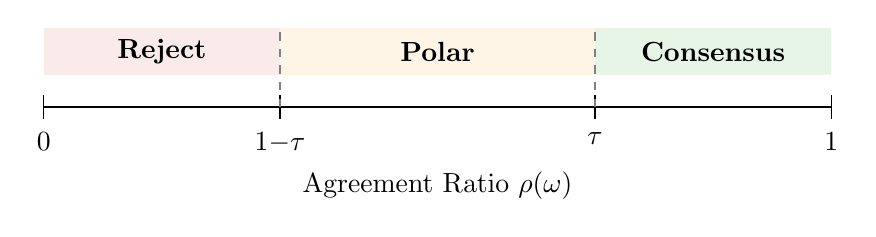
\begin{tikzpicture}[scale=1]
    % Number line
    \draw[thick, -] (0,0) -- (10,0);
    
    % Tick marks
    \foreach \x/\label in {0/0, 3/$1{-}\tau$, 7/$\tau$, 10/1} {
        \draw (\x, 0.15) -- (\x, -0.15);
        \node[below] at (\x, -0.2) {\label};
    }
    
    % Regions
    \fill[cullbg] (0,0.4) rectangle (3,1.0);
    \fill[polarbg] (3,0.4) rectangle (7,1.0);
    \fill[consensusbg] (7,0.4) rectangle (10,1.0);
    
    % Region labels
    \node at (1.5, 0.7) {\textbf{Reject}};
    \node at (5, 0.7) {\textbf{Polar}};
    \node at (8.5, 0.7) {\textbf{Consensus}};
    
    % Axis label
    \node[below] at (5, -0.7) {Agreement Ratio $\rho(\omega)$};
    
    % Boundaries
    \draw[dashed, gray] (3, 0) -- (3, 1.0);
    \draw[dashed, gray] (7, 0) -- (7, 1.0);
\end{tikzpicture}
\end{center}

\vspace{1em}

The threshold $\tau$ controls the boundaries symmetrically:
\begin{itemize}[noitemsep]
    \item Higher $\tau$ (e.g., $0.8$) → stricter consensus requirement, wider Polar band
    \item Lower $\tau$ (e.g., $0.6$) → more permissive consensus, narrower Polar band
    \item $\tau = 0.5$ → no Polar tier (binary: Consensus or Reject)
    \item $\tau = 1.0$ → only unanimous approval counts as Consensus
\end{itemize}

\subsection{Tier Definitions}

\begin{greenbox}[Consensus \normalfont{— $\rho(\omega) \geq \tau$}]
A strong majority of clusters approve. This artifact resonates across adversarial perspectives and represents robust agreement.\\[0.5em]
\textbf{Action: GROUND} — Use as primary context for response synthesis.\\[0.5em]
\textit{Special case:} When $|S(\omega)| = n$ (all clusters approve), this is \textbf{Full Consensus}—the highest confidence level. The orchestrator may flag this distinction.
\end{greenbox}

\begin{orangebox}[Polar \normalfont{— $1 - \tau < \rho(\omega) < \tau$}]
Mixed approval—some clusters approve, others reject. This artifact is contested; it may represent a valid perspective but not cross-cutting agreement.\\[0.5em]
\textbf{Action: CONTEXTUALIZE} — Include with attribution to approving clusters.
\end{orangebox}

\begin{redbox}[Reject \normalfont{— $\rho(\omega) \leq 1 - \tau$}]
A strong majority of clusters reject. This artifact fails cross-examination and should be discarded.\\[0.5em]
\textbf{Action: EXCLUDE} — Do not include in response synthesis.
\end{redbox}

\subsection{Note on Empty Tiers}

For small $n$ or certain values of $\tau$, the Polar tier may be empty (no discrete $\rho$ values fall in the range). This is expected behavior, not an error—it simply means the system operates in binary mode for that configuration.

%----------------------------------------------------------
\section{The Binary Case ($n = 2$)}
%----------------------------------------------------------

The most common configuration uses two adversarial clusters. This section illustrates the framework with $n = 2$.

\subsection{Setup}

Let $\mathcal{C} = \{C^+, C^-\}$ represent two opposing perspectives (e.g., advocate and critic). The approval set $S(\omega)$ can take four values:

\begin{center}
\begin{tabular}{@{}cccc@{}}
\toprule
$S(\omega)$ & $|S|$ & $\rho$ & Interpretation \\
\midrule
$\{C^+, C^-\}$ & 2 & 1.0 & Both clusters approve \\
$\{C^+\}$ & 1 & 0.5 & Only advocates approve \\
$\{C^-\}$ & 1 & 0.5 & Only critics approve \\
$\emptyset$ & 0 & 0.0 & Neither approves \\
\bottomrule
\end{tabular}
\end{center}

\subsection{Classification with $\tau = 0.6$}

\begin{center}
\begin{tabular}{@{}cccl@{}}
\toprule
$S(\omega)$ & $\rho$ & Tier & Action \\
\midrule
$\{C^+, C^-\}$ & 1.0 & Consensus & GROUND \\
$\{C^+\}$ & 0.5 & Polar & CONTEXTUALIZE as advocate position \\
$\{C^-\}$ & 0.5 & Polar & CONTEXTUALIZE as critic position \\
$\emptyset$ & 0.0 & Reject & EXCLUDE \\
\bottomrule
\end{tabular}
\end{center}

\subsection{The 2×2 Quadrant View}

For $n = 2$, the classification can be visualized as a quadrant:

\begin{center}
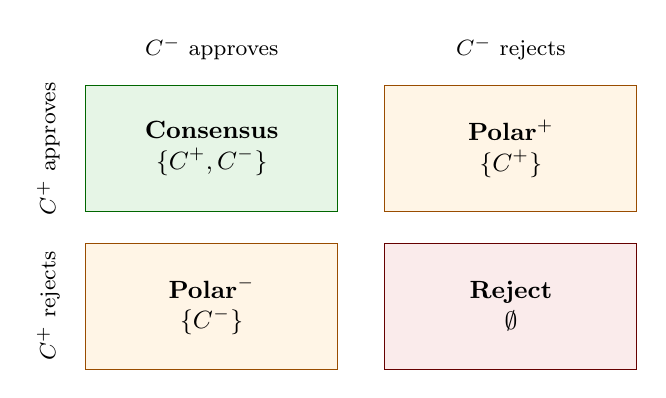
\begin{tikzpicture}[
    box/.style={rectangle, minimum width=3.2cm, minimum height=1.6cm, align=center, font=\small},
]
    \node[box, fill=consensusbg, draw=green!40!black] (q11) at (0, 0) {\textbf{Consensus}\\$\{C^+, C^-\}$};
    \node[box, fill=polarbg, draw=orange!60!black] (q10) at (3.8, 0) {\textbf{Polar}$^+$\\$\{C^+\}$};
    \node[box, fill=polarbg, draw=orange!60!black] (q01) at (0, -2.0) {\textbf{Polar}$^-$\\$\{C^-\}$};
    \node[box, fill=cullbg, draw=red!40!black] (q00) at (3.8, -2.0) {\textbf{Reject}\\$\emptyset$};
    
    \node[above=0.2cm of q11, font=\footnotesize] {$C^-$ approves};
    \node[above=0.2cm of q10, font=\footnotesize] {$C^-$ rejects};
    \node[left=0.2cm of q11, font=\footnotesize, rotate=90, anchor=south] {$C^+$ approves};
    \node[left=0.2cm of q01, font=\footnotesize, rotate=90, anchor=south] {$C^+$ rejects};
\end{tikzpicture}
\end{center}

%----------------------------------------------------------
\section{Scoring}
%----------------------------------------------------------

Within each tier, artifacts are ranked by \textbf{total approval rate}:

\begin{equation}
\text{Score}(\omega) = \frac{1}{|\mathcal{A}| - 1} \sum_{a \neq \text{author}(\omega)} v(\omega, a)
\end{equation}

This is the fraction of non-authoring agents who approved, regardless of cluster. Higher scores indicate stronger overall support.

\subsection{Optional: Consensus Balance Bonus}

For Consensus artifacts, balanced approval across clusters may be preferred. An optional refinement penalizes lopsided agreement:

\begin{equation}
\text{Score}_{\text{balanced}}(\omega) = \text{Score}(\omega) \times \left(1 - \sigma_S(\omega)\right)
\end{equation}

Where $\sigma_S(\omega)$ is the standard deviation of per-cluster approval rates:

\begin{equation}
\sigma_S(\omega) = \sqrt{\frac{1}{n} \sum_{i=1}^{n} \left(r_i(\omega) - \bar{r}(\omega)\right)^2}
\end{equation}

And $r_i(\omega) = \frac{1}{|C_i|} \sum_{a \in C_i} v(\omega, a)$ is the approval rate within cluster $C_i$.

%----------------------------------------------------------
\section{Persuasive Artifacts}
%----------------------------------------------------------

A valuable subclass of Consensus artifacts demonstrate \textbf{cross-cluster persuasion}: they were authored by one cluster but approved by adversarial clusters.

\begin{defbox}[Cross-Cluster Persuasion]
For a Consensus artifact $\omega$ authored by an agent in cluster $C_i$:
\begin{itemize}[noitemsep, topsep=0pt]
    \item The artifact is \textbf{persuasive} if $C_j \in S(\omega)$ for some $j \neq i$
    \item The \textbf{persuasion reach} is $|S(\omega) \setminus \{C_i\}|$ — how many adversarial clusters it convinced
\end{itemize}
\end{defbox}

For $n = 2$, this simplifies to:
\begin{itemize}[noitemsep]
    \item \textbf{Accelerator}: Consensus artifact authored by $C^+$, approved by $C^-$ \\ {\small\itshape ``An advocate's argument that even critics accept.''}
    \item \textbf{Mitigator}: Consensus artifact authored by $C^-$, approved by $C^+$ \\ {\small\itshape ``A critic's argument that even advocates acknowledge.''}
\end{itemize}

These are high-value artifacts for constructing balanced responses.

%----------------------------------------------------------
\section{The Contextual Superposition}
%----------------------------------------------------------

The protocol outputs a \textbf{Contextual Superposition} for each artifact—a structured summary for the orchestrator:

\begin{defbox}[Superposition Object]
\begin{verbatim}
Superposition(ω) = {
    artifact: ω,
    approval_set: S(ω),
    agreement_ratio: ρ(ω),
    tier: Consensus | Polar | Reject,
    score: Score(ω),
    author_cluster: C_i,
    is_persuasive: boolean,
    full_consensus: boolean  // true if |S| = n
}
\end{verbatim}
\end{defbox}

The orchestrator receives a list of these objects, grouped by tier and sorted by score.

%----------------------------------------------------------
\section{Orchestrator Actions}
%----------------------------------------------------------

\begin{center}
\begin{tabular}{@{}llp{6.5cm}@{}}
\toprule
\textbf{Tier} & \textbf{Action} & \textbf{Guidance} \\
\midrule
Consensus (Full) & \textsc{Ground} & Highest confidence. Lead with these points. \\
Consensus (Partial) & \textsc{Ground} & High confidence. Note dissenting clusters if relevant. \\
Polar & \textsc{Contextualize} & Include with attribution: ``From [cluster] perspective...'' \\
Reject & \textsc{Exclude} & Do not reference. \\
\addlinespace
Persuasive & \textsc{Emphasize} & Strong bridge-building points. \\
\bottomrule
\end{tabular}
\end{center}

%----------------------------------------------------------
\section{Algorithm}
%----------------------------------------------------------

\begin{algorithm}[H]
\caption{Resonant Consensus Protocol}
\begin{algorithmic}[1]
\Require Agents $\mathcal{A}$ partitioned into clusters $\mathcal{C} = \{C_1, \ldots, C_n\}$
\Require Query $q$, thresholds $\theta$ (cluster approval), $\tau$ (consensus)
\Ensure List of Superposition objects for orchestrator
\State
\State \textbf{// Phase 1: Generate}
\For{each $a \in \mathcal{A}$}
    \State $\omega_a \gets a.\text{respond}(q)$
\EndFor
\State $\Omega \gets \{\omega_a : a \in \mathcal{A}\}$
\State
\State \textbf{// Phase 2: Vote}
\For{each $\omega \in \Omega$}
    \For{each $a \in \mathcal{A}$ where $a \neq \text{author}(\omega)$}
        \State $v(\omega, a) \gets a.\text{approve}(\omega)$ \Comment{Returns 0 or 1}
    \EndFor
\EndFor
\State
\State \textbf{// Phase 3: Classify}
\For{each $\omega \in \Omega$}
    \For{each $C_i \in \mathcal{C}$}
        \State $r_i \gets \frac{1}{|C_i|} \sum_{a \in C_i} v(\omega, a)$
        \State $\text{Approve}_i(\omega) \gets \mathbf{1}[r_i \geq \theta_i]$
    \EndFor
    \State $S(\omega) \gets \{C_i : \text{Approve}_i(\omega) = 1\}$
    \State $\rho(\omega) \gets |S(\omega)| / n$
    \State
    \If{$\rho(\omega) \geq \tau$}
        \State $\text{tier} \gets \textsc{Consensus}$
    \ElsIf{$\rho(\omega) > 1 - \tau$}
        \State $\text{tier} \gets \textsc{Polar}$
    \Else
        \State $\text{tier} \gets \textsc{Reject}$
    \EndIf
    \State
    \State Compute $\text{Score}(\omega)$
    \State Build Superposition object
\EndFor
\State
\State \textbf{// Phase 4: Return}
\State Sort by tier (Consensus $>$ Polar $>$ Reject), then by Score descending
\State \Return list of Superposition objects
\end{algorithmic}
\end{algorithm}

%----------------------------------------------------------
\section{Implementation Notes}
%----------------------------------------------------------

\subsection{Eliciting Votes}

Prompt each agent:
\begin{quote}
\texttt{Given your perspective, does this response represent sound}\\
\texttt{reasoning you would endorse? Answer YES or NO.}\\[0.5em]
\texttt{Response to evaluate: [artifact text]}
\end{quote}

Map YES $\to 1$, NO $\to 0$.

\subsection{Minimum Panel Size}

Each cluster requires $\geq 2$ agents for meaningful approval rates. With exactly 2 agents per cluster, $\theta = 0.5$ requires both to agree (unanimous within cluster).

Recommended minimum: 3 agents per cluster.

\subsection{Parameter Defaults}

\begin{center}
\begin{tabular}{@{}lll@{}}
\toprule
Parameter & Default & Meaning \\
\midrule
$\theta$ & $0.5$ & Simple majority within cluster \\
$\tau$ & $0.6$ & 60\% of clusters required for Consensus \\
\bottomrule
\end{tabular}
\end{center}

%----------------------------------------------------------
\section{Extensions}
%----------------------------------------------------------

\subsection{Per-Cluster Thresholds}

Different clusters may warrant different approval thresholds. For example, a ``safety reviewer'' cluster might require $\theta_{\text{safety}} = 0.9$ (near-unanimous) while others use $\theta = 0.5$.

Set $\theta_i$ individually, or use the global default:
\begin{equation}
\theta_i = \theta_{\text{global}} \quad \text{for all } i \quad \text{(default behavior)}
\end{equation}

\subsection{Weighted Clusters}

If some clusters are more authoritative, weight their approval:
\begin{equation}
\rho_{\text{weighted}}(\omega) = \frac{\sum_{C_i \in S(\omega)} w_i}{\sum_{i=1}^{n} w_i}
\end{equation}

Where $w_i$ is the weight of cluster $C_i$. This allows, e.g., domain experts to have more influence than general reviewers.

\subsection{Iterative Refinement}

For complex queries, iterate:
\begin{enumerate}[noitemsep]
    \item Run the protocol
    \item Use Consensus artifacts as context for a second generation round
    \item Re-evaluate and re-classify
\end{enumerate}

This allows agents to refine positions based on verified common ground.

%----------------------------------------------------------
\section{Summary}
%----------------------------------------------------------

The Resonant Consensus Protocol classifies multi-agent outputs by cross-cluster agreement:

\begin{enumerate}[noitemsep]
    \item Partition agents into $n$ adversarial clusters
    \item Collect binary approval votes on each artifact
    \item Compute approval set $S(\omega)$ and agreement ratio $\rho(\omega)$
    \item Classify into Consensus / Polar / Reject based on threshold $\tau$
    \item Return Contextual Superposition to orchestrator
\end{enumerate}

The key insight: \textbf{who agrees matters as much as how many agree}. An artifact with 60\% approval is Consensus if that support spans clusters, but Polar if concentrated in one. This distinction enables orchestrators to separate robust insights from tribal bias.

\vspace{2em}

%----------------------------------------------------------
\section*{Quick Reference}
%----------------------------------------------------------

\begin{center}
\begin{tabular}{@{}ll@{}}
\toprule
\textbf{Symbol} & \textbf{Definition} \\
\midrule
$\mathcal{C} = \{C_1, \ldots, C_n\}$ & Set of adversarial clusters \\
$v(\omega, a)$ & Binary vote: agent $a$ approves artifact $\omega$ \\
$\theta_i$ & Approval threshold for cluster $C_i$ \\
$S(\omega)$ & Approval set: clusters that approve $\omega$ \\
$\rho(\omega) = |S(\omega)|/n$ & Agreement ratio \\
$\tau$ & Consensus threshold \\
\bottomrule
\end{tabular}
\end{center}

\vspace{1em}

\begin{center}
\begin{tabular}{@{}lll@{}}
\toprule
\textbf{Condition} & \textbf{Tier} & \textbf{Action} \\
\midrule
$\rho \geq \tau$ & Consensus & \textsc{Ground} \\
$1 - \tau < \rho < \tau$ & Polar & \textsc{Contextualize} \\
$\rho \leq 1 - \tau$ & Reject & \textsc{Exclude} \\
\bottomrule
\end{tabular}
\end{center}

\end{document}
